\documentclass[
  french,
  a4paper,
]{scrartcl}

\usepackage[pages=some]{background}
%\ULCornerWallPaper{1}{arc-template.pdf}
\backgroundsetup{firstpage = true, scale = 1, angle = 0, opacity = 1, 
contents = {
\includegraphics[width = \paperwidth, height = \paperheight] {arc-template.pdf}}}

\usepackage{listings}
\usepackage{tabularray}
\usepackage{array}
\usepackage{rotating}

\usepackage{xcolor}
\definecolor{codegreen}{rgb}{0,0.6,0}
\definecolor{codegray}{rgb}{0.5,0.5,0.5}
\definecolor{codepurple}{rgb}{0.58,0,0.82}
\definecolor{backcolour}{rgb}{0.98,0.98,0.98}

\lstdefinestyle{mystyle}{
    backgroundcolor=\color{backcolour},   
    commentstyle=\color{codegreen},
    keywordstyle=\color{magenta},
    numberstyle=\tiny\color{codegray},
    stringstyle=\color{codepurple},
    basicstyle=\ttfamily\footnotesize,
    breakatwhitespace=false,         
    breaklines=true,                 
    captionpos=b,                    
    keepspaces=true,                 
    numbers=left,                    
    numbersep=5pt,                  
    showspaces=false,                
    showstringspaces=false,
    showtabs=false,                  
    tabsize=2
}
\lstset{style=mystyle}

\usepackage{amsmath,amssymb}
\usepackage[french]{babel}

\usepackage[T1]{fontenc}
\usepackage[utf8]{inputenc}

\usepackage{lmodern}

\usepackage{xcolor}
\usepackage[margin=2cm,includehead,includefoot]{geometry}
\usepackage{longtable,booktabs,array}
\usepackage{calc}
\usepackage[hidelinks]{hyperref}
\usepackage{etoolbox}

\renewcommand{\arraystretch}{1.2}
\setlength {\parindent}{0em}
\setlength {\parskip}{1em}

\usepackage{fancyhdr}
\pagestyle{fancy}

\title{Laboratoire 1 : Analyse et comparaison de performances 
entre une recherche linéaire et une recherche concurrente en Java}
\subject{3259.1 Paradigmes de programmation avancés II $\cdot$ ISC3il-a}
\author{Nima Dekhli\\
    \small \href{mailto:nima.dekhli@he-arc.ch}{nima.dekhli@he-arc.ch}}
\date{\today}


\makeatletter
\providecommand{\subtitle}[1]{% add subtitle to \maketitle
  \apptocmd{\@title}{\par {\large #1 \par}}{}{}
}
\makeatother


\begin{document}
\maketitle
\tableofcontents

\section{Introduction}

Dans le cadre du cours de paradigmes de programmation avancés II, il nous 
a été demandé de réaliser un laboratoire qui consiste à comparer les performances
de deux algorithmes de recherche, à savoir la recherche linéaire et la recherche
concurrente. La recherche concurrente est une recherche dichotomique qui est
exécutée en parallèle sur plusieurs Threads, en utilisant un ForkJoinPool.

La recherche s'effectue sur une base de données de films qui nous a été fournie. 
Les méthodes de chargement de la base de données, ainsi que le filtrage 
pour la recherche ont été fournies. Il nous a été demandé de spécifiquement réaliser
la partie de recherche. 

Ce rapport présente la comparaison de performances entre ces deux algorithmes, 
ainsi que l'impact sur la performance du nombre de découpages 
lors de la recherche concurrente.

\section{Implémentation}

\subsection{Recherche linéaire}

La recherche linéaire est effectuée dans la classe 
\lstinline|LinSearch|. Son implémentation est assez simple : 
elle parcourt la base de données, sous forme de tableau, du premier élément 
au dernier et applique la méthode de filtrage sur chacun d'entre eux. 
Cette méthode de filtrage est fournie par la méthode \lstinline|Filtre.filtre()|.
Elle prend en paramètre un élément de la base de données ainsi que la liste des filtres
à appliquer et retourne un booléen indiquant si l'élément correspond aux filtres. 

Dans le cas de la recherche d'un seul élément (méthode \lstinline|LinSearch.trouve()|), après 
avoir trouvé le premier élément correspondant aux filtres, la recherche s'arrête 
immédiatement. 

Dans le cas de la recherche de tous les éléments (méthode \lstinline|LinSearch.trouveTous()|),
à chaque fois qu'un élément correspondant aux filtres est trouvé, il est ajouté à
une liste qui est retournée à la fin de la recherche, quand tous les éléments ont été
parcourus.

\subsection{Recherche concurrente}

La recherche concurrente est effectuée dans la classe \lstinline|ConcSearch|.
Elle utilise un ForkJoinPool pour exécuter la recherche en parallèle sur plusieurs Threads.

Chaque tâche récursive, implémentée par la classe \lstinline|FindTask|, étend la 
classe abstraite \lstinline|RecursiveAction|. La méthode \lstinline|compute()| est 
implémentée pour effectuer la recherche. 

La recherche est effectuée de manière dichotomique : tant que l'intervalle de recherche 
de la tâche courante est plus grand que le \textit{batch size}, alors la tâche 
est divisée en deux sous-tâches qui sont exécutées en parallèle, grâce 
à la méthode \lstinline{FindTask.fork()}. La fin de l'exécution des sous-tâches 
est attendue grâce à la méthode \lstinline{FindTask.join()}.

Une fois que les deux sous-tâches sont terminées, les résultats sont récupérés 
et la variable \lstinline|result| est mise à jour. 

Dans le cas de la recherche d'un seul élément (méthode \lstinline|ConcSearch.trouve()|),
il est nécessaire d'arrêter la recherche lorsque un élément correspondant aux filtres
est trouvé. La méthode s'exécutant en parallèle, il s'avère plus complexe que 
dans le cas de la recherche linéaire. Dans le cas le plus simple, 
après avoir trouvé un élément, on quitte immédiatement la tâche courante. 
Toutefois, toutes les autres tâches qui ont été lancées doivent également être 
arrêtées.

Pour cela, la solution qui a été choisie est d'ajouter un \textit{flag} statique \lstinline|found|
de type \lstinline|AtomicBoolean|. Comme la variable est statique, elle est partagée
entre toutes les tâches (d'où l'intérêt d'utiliser un \lstinline|AtomicBoolean|).
La vérification du flag est effectuée à deux endroits : premièrement, tout au début de
 la tâche et deuxièmement, pendant la recherche, toutes les 
100 itérations. 
Si au moment de ces vérifications, le flag est à \lstinline|true|, alors la tâche 
courante est arrêtée.

Ce mécanisme permet ainsi aux tâches en cours d'être rapidement informées
si une autre tâche a déjà trouvé le résultat recherché. 


\section{Résultats}

\subsection{Motivation}

Nous souhaitons comparer les performances de la recherche linéaire et de la 
recherche concurrente. De plus, nous souhaitons également étudier l'impact
du nombre de découpages en tâches parallèles, sur la performance de la 
recherche concurrente. La performance est mesurée en termes de temps d'exécution.

\subsection{Protocole de tests}

Pour obtenir des résultats fiables, chaque mesure a été effectuée 1000 fois de suite et 
le temps d'exécution médian a été retenu. Étant donné que le nombre de valeurs 
dans le dataset est de 722'625, 13 valeurs de batch sizes choisies entre 1'000'000 et 1. 
De cette manière, le nombre de Threads varie entre 1 (recherche linéaire) et env. 700'000 
(1 thread par case). 

Sur la table \ref{tab:batch}, est représenté le nombre de découpages successifs, 
la taille des batch réelle et le nombre de Threads en fonction de la taille du batch choisie. 
Le nombre de Threads indiqué correspond à ceux qui effectueront la recherche linéaire (les feuilles
de l'arbre). Toutefois, il faut noter que le nombre de Threads effectivement utilisés
est plus grand (les nœuds de l'arbre).

\begin{table}[h]
  \centering
  \begin{tabular}{|l|l|l|l|}
    \hline
    \textbf{taille du batch (max)}  & \textbf{découpages} & \textbf{taille réelle approx.} & \textbf{nombre de Threads}\\
    \hline\hline
    1'000'000 & 0 & 722'625 & 1\\
    \hline
    500'000 & 1 & 361'312 & 2\\
    \hline
    100'000 & 3& 90'328 & 8\\
    \hline 
    50'000 & 4 & 45'164 & 16\\
    \hline
    10'000 & 7 & 5'645 & 128\\
    \hline
    5'000 & 8 & 2822 & 256\\
    \hline
    1000 & 10 & 705 & 1'024\\
    \hline
    100 & 13 & 88 & 8'192\\
    \hline 
    50 & 14 & 44 & 16'384\\
    \hline
    10 & 17 & 6 & 131'072\\
    \hline 
    5 & 18 & 3 & 262'144\\
    \hline
    2 & 19 & 2 & 361'312\\
    \hline
    1 & 20 & 1 & 722'625\\
    \hline
    
  \end{tabular}
  \caption{Nombre de découpages et nombre de Threads en fonction de la taille du batch}
  \label{tab:batch}
\end{table}


Les deux machines utilisées pour les tests sont un \textit{MacBook Pro 14" M2 Pro Early 2023} 
et un \textit{Dell XPS 15 9500}. Les spécifications de ces machines sont résumées dans 
les tables \ref{tab:spec-dell} et \ref{tab:spec-mac}.


\begin{table}[h]
  \centering
\begin{tabular}[pos]{|l|l|}
  \hline
  \textbf{Attribut} & \textbf{Valeur} \\
  \hline\hline
  Famille CPU & Intel Core i7 10th Gen \\
  \hline
  Modèle CPU & i7-10750H \\
  \hline
  Architecture & x86\_64 (AMD64)\\
  \hline
  Nb cœurs total & 12 \\
  \hline
  RAM & 32 Go \\
  \hline
  Stockage & SSD M.2\\
  \hline
  OS & Ubuntu 22.04.3 LTS\\
  \hline
  Kernel & Linux 5.15.0-86-generic\\
  \hline
\end{tabular}
\caption{Spécifications de la machine \textit{Dell XPS 15 9500}}
\label{tab:spec-dell}
\end{table}
  
\begin{table}[h]
  \centering
\begin{tabular}[pos]{|l|l|}
  \hline
  \textbf{Attribut} & \textbf{Valeur} \\
  \hline\hline
  Famille CPU & Apple Silicon\\
  \hline
  Modèle CPU &  Apple M2 Pro \\
  \hline
  Architecture & AArch64 (ARM64)\\
  \hline
  Nb cœurs total & 10\\
  \hline
  RAM & 16 Go \\
  \hline
  Stockage & SSD \\
  \hline
  OS & macOS 14.3.1 (23D60)\\
  \hline
  Kernel & Darwin 23.3.0\\
  \hline
\end{tabular}
\caption{Spécifications de la machine \textit{MacBook Pro 14" M2 Pro Early 2023}}
\label{tab:spec-mac}
\end{table}

\subsection{Mesures}

Les résultats des mesures de performances sur la machine \textit{Dell XPS 15 9500} 
sont présentés dans les tables \ref{tab:measure-linux-conc} et \ref{tab:measure-linux-lin}, 
tandis que les résultats sur la machine \textit{MacBook Pro 14" M2 Pro Early 2023}
sont présentés dans les tables \ref{tab:measure-mac-conc} et \ref{tab:measure-mac-lin}.

Sur les figures \ref{fig:result-linux} et \ref{fig:result-mac} sont représentées
mesures de performances sous forme graphique pour les deux machines. 

\begin{table}[h]
  \centering
  \begin{tblr}{
      |l|l|l|l|l|
  }
  \hline
  \textbf{batch size}   & \textbf{test1} & \textbf{test2} & \textbf{test3} & \textbf{test5}  \\
  \hline\hline
  \textbf{1000000} & 0.0774         & 46.56052       & 63.198937      & 64.232979       \\
  \hline
  \textbf{500000}  & 0.109278       & 27.536158      & 37.217301      & 39.325117       \\
  \hline
  \textbf{100000}  & 0.087939       & 20.264994      & 27.225019      & 25.002329       \\
  \hline
  \textbf{50000}   & 0.087448       & 18.298418      & 23.6877        & 22.013021       \\
  \hline
  \textbf{10000}   & 0.079751       & 16.909785      & 24.533562      & 20.909389       \\
  \hline
  \textbf{5000}    & 0.076145       & 16.242429      & 24.309161      & 20.839093       \\
  \hline
  \textbf{1000}    & 0.071714       & 16.795871      & 24.369978      & 20.794897       \\
  \hline
  \textbf{100}     & 0.072483       & 14.85043       & 24.053301      & 20.147315       \\
  \hline
  \textbf{50}      & 0.071205       & 14.153743      & 23.029809      & 19.592804       \\
  \hline
  \textbf{10}      & 0.069307       & 11.317111      & 18.408586      & 17.685128       \\
  \hline
  \textbf{5}       & 0.070649       & 12.328179      & 18.585123      & 18.252072       \\
  \hline
  \textbf{2}       & 0.070806       & 17.087922      & 22.957968      & 23.305204       \\
  \hline
  \textbf{1}       & 0.072062       & 21.804465      & 28.280596      & 28.536901       \\
  \hline
  \end{tblr}
  \caption[Performances en mode concurrent sur \textit{Dell XPS 15 9500}]{Temps d'exécution en millisecondes pour chaque test en fonction du batch size sur
  la machine \textit{Dell XPS 15 9500} en mode concurrent}
  \label{tab:measure-linux-conc}
  \end{table}
  
\begin{table}[h]
  \centering
  \begin{tblr}{
      |l|l|l|l|l|
  }
  \hline
  \textbf{test1} & \textbf{test2} & \textbf{test3} & \textbf{test5}   \\
  \hline
  0.00152        & 44.54128       & 62.996274      & 65.374348        \\
  \hline
  \end{tblr}
  \caption[Performances en mode linéaire sur \textit{Dell XPS 15 9500}]{Temps d'exécution en millisecondes pour chaque test sur
  la machine \textit{Dell XPS 15 9500} en mode linéaire}
  \label{tab:measure-linux-lin}
  \end{table} 
  
  \begin{figure}[h]
    \centering
    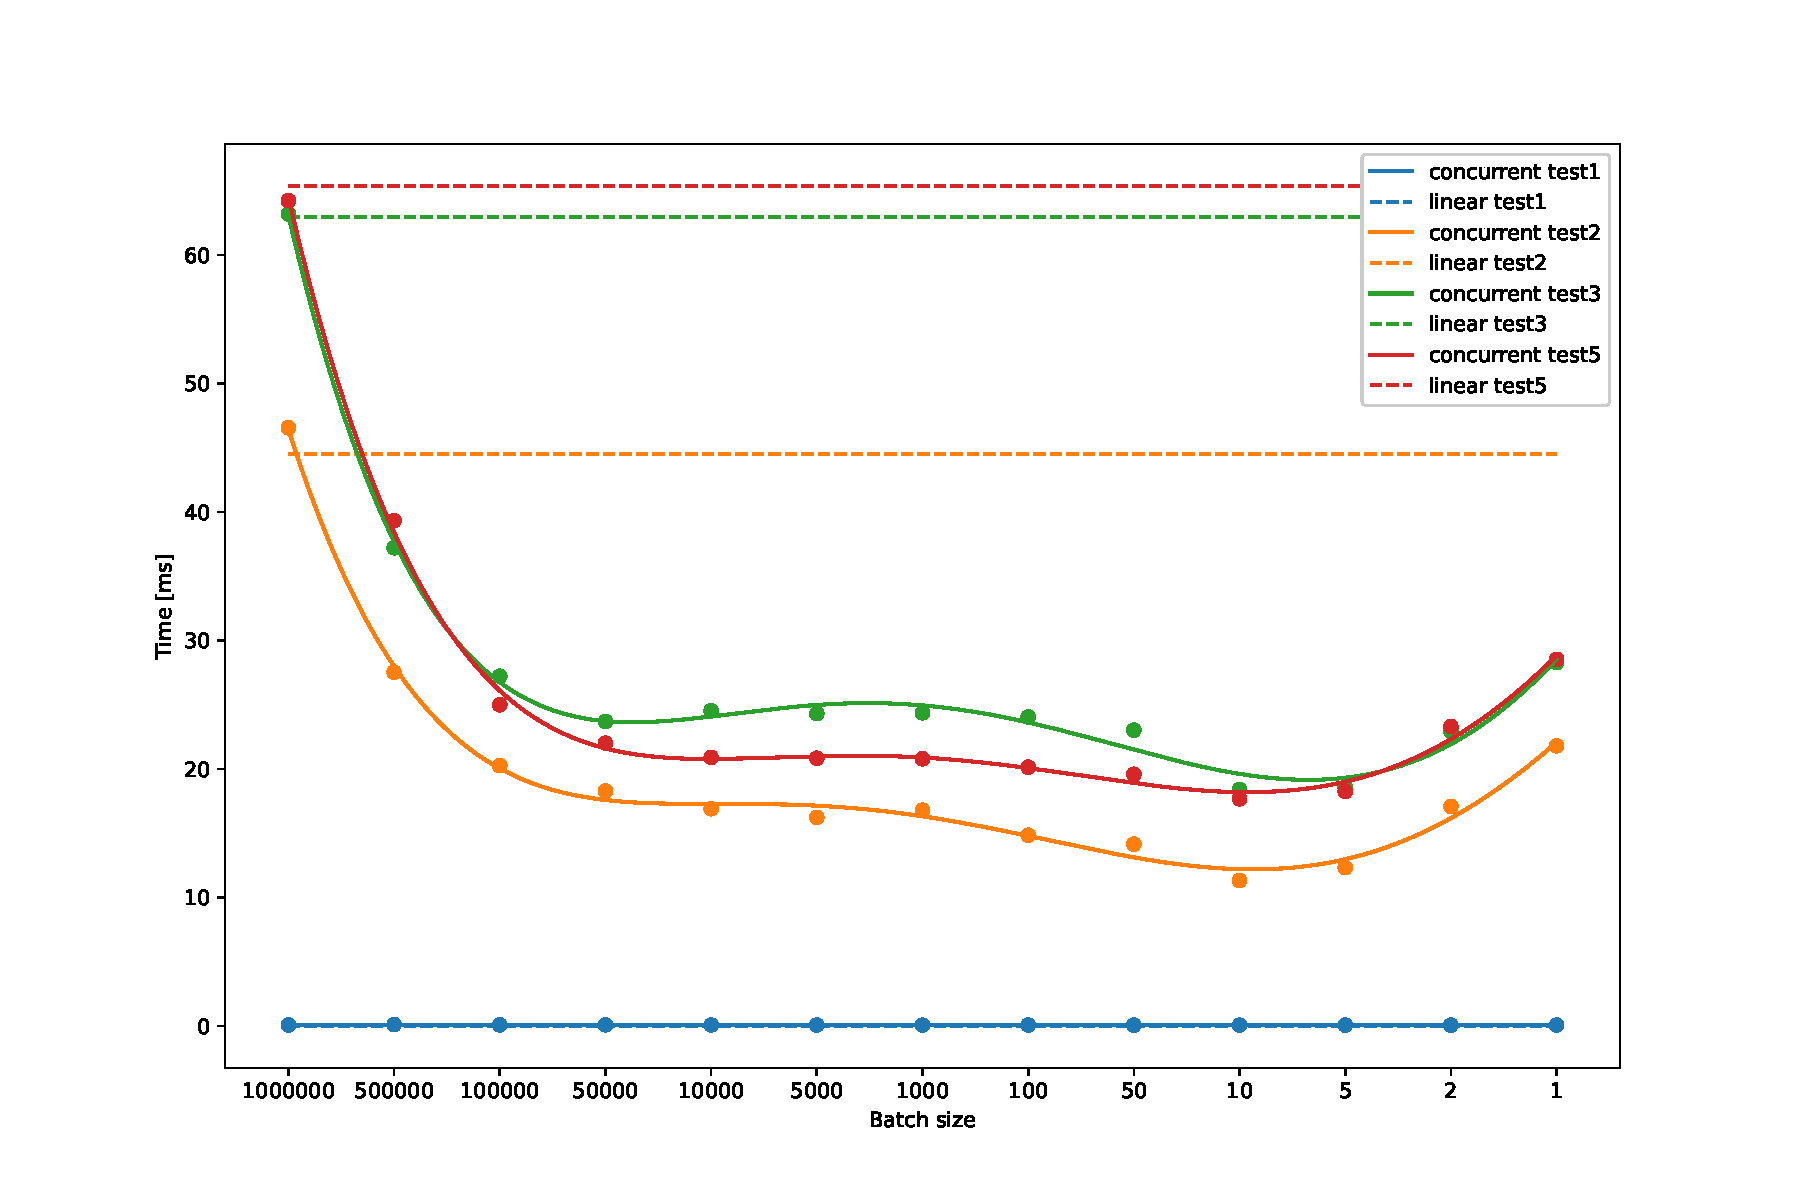
\includegraphics[width=\textwidth]{assets/result-linux.pdf}
    \caption[Graphique des performances sur \textit{Dell XPS 15 9500}]{Représentation graphiques des mesures de performances sur la machine \textit{Dell XPS 15 9500}}
    \label{fig:result-linux}
  \end{figure}

\begin{table}[h]
  \centering
  \begin{tblr}{
      |l|l|l|l|l|
  }
  \hline
  \textbf{batch size}   & \textbf{test1} & \textbf{test2} & \textbf{test3} & \textbf{test5}   \\
  \hline\hline
  \textbf{1000000} & 0.059083       & 37.653         & 43.840667      & 49.716042        \\
  \hline
  \textbf{500000}  & 0.083875       & 19.629083      & 23.807875      & 24.4             \\
  \hline
  \textbf{100000}  & 0.090292       & 8.953          & 10.28725       & 11.056125        \\
  \hline
  \textbf{50000}   & 0.085958       & 6.51325        & 8.763292       & 10.381084        \\
  \hline
  \textbf{10000}   & 0.086917       & 6.2555         & 8.450583       & 9.473333         \\
  \hline
  \textbf{5000}    & 0.083          & 6.262458       & 8.301459       & 8.89275          \\
  \hline
  \textbf{1000}    & 0.073584       & 6.261833       & 7.897792       & 9.085708         \\
  \hline
  \textbf{100}     & 0.077542       & 6.494458       & 8.019375       & 8.63775          \\
  \hline
  \textbf{50}      & 0.082459       & 6.308375       & 8.297375       & 8.906084         \\
  \hline
  \textbf{10}      & 0.07875        & 7.809792       & 9.773625       & 10.149791        \\
  \hline
  \textbf{5}       & 0.082083       & 8.96725        & 10.976583      & 11.843417        \\
  \hline
  \textbf{2}       & 0.078167       & 11.276125      & 14.4925        & 14.620209        \\
  \hline
  \textbf{1}       & 0.075708       & 15.46225       & 19.052208      & 20.215958       \\ 
  \hline
  \end{tblr}
  
  \caption[Performances en mode concurrent sur \textit{MacBook Pro 14" M2 Pro Early 2023}]{Temps d'exécution en millisecondes pour chaque test en fonction du batch size sur 
  la machine \textit{MacBook Pro 14" M2 Pro Early 2023} en mode concurrent}
  \label{tab:measure-mac-conc}
  \end{table}

\begin{table}[h]
  \centering
  \begin{tblr}{
      |l|l|l|l|l|
  }
  \hline
  \textbf{test1} & \textbf{test2} & \textbf{test3} & \textbf{test5} \\
  \hline
  0.001291       & 28.339708      & 32.609167      & 42.11875       \\
  \hline
  \end{tblr}
  \caption[Performances en mode linéaire sur \textit{MacBook Pro 14" M2 Pro Early 2023}]{Temps d'exécution en millisecondes pour chaque test sur
  la machine \textit{MacBook Pro 14" M2 Pro Early 2023} en mode linéaire}
  \label{tab:measure-mac-lin}
  \end{table} 
  
  \begin{figure}[h]
    \centering
    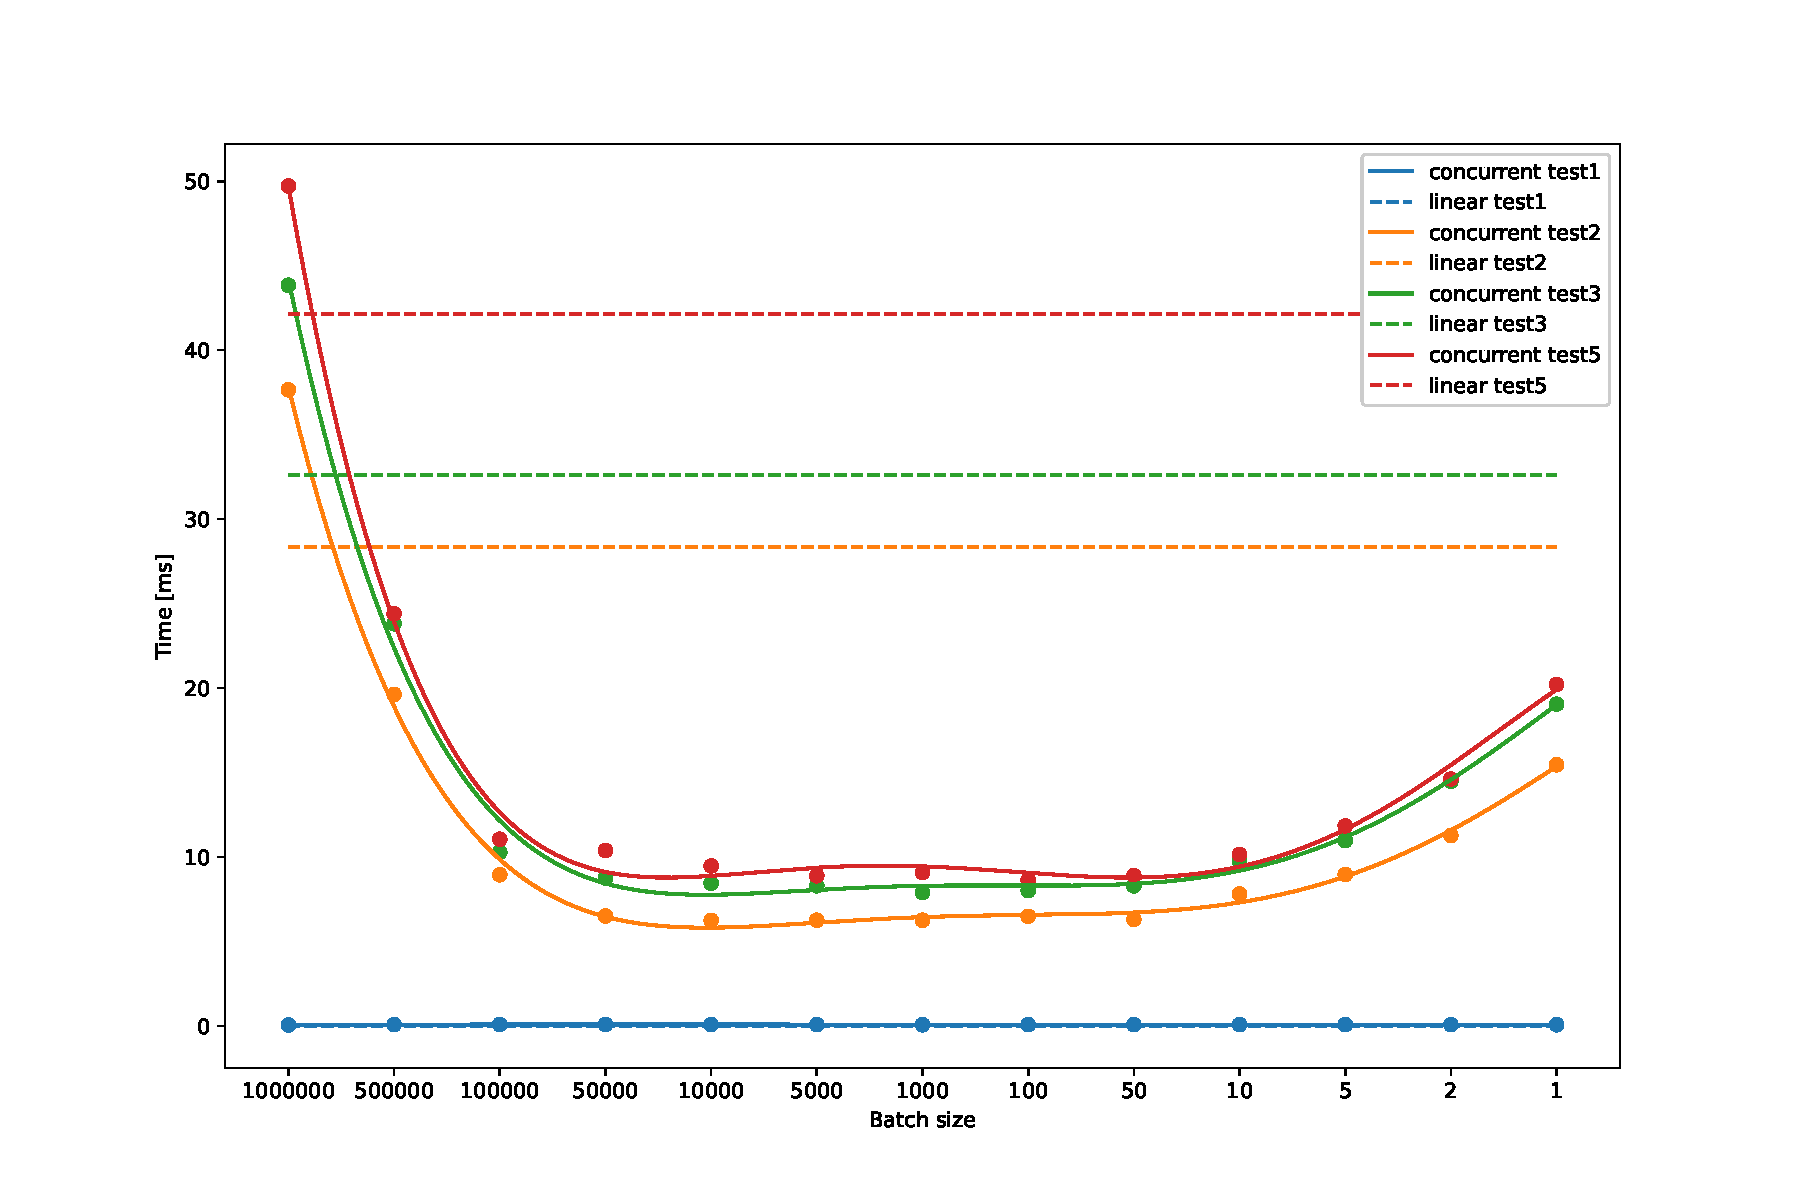
\includegraphics[width=\textwidth]{assets/result-mac.pdf}
    \caption[Graphique des performances sur \textit{MacBook Pro 14" M2 Pro Early 2023}]{Représentation graphique des mesures de performances sur la machine \textit{MacBook Pro 14" M2 Pro Early 2023}}
    \label{fig:result-mac}
  \end{figure}

\section{Analyse}

\subsection{Comparaison entre le mode linéaire et le mode concurrent}

Les tests montrent que sur les deux machines de test, le mode concurrent est plus rapide
que le mode linéaire, sauf pour le test 1. En effet, il se trouve que l'élément à rechercher 
est au tout début de la base de données. Dans ce cas, la recherche linéaire est plus rapide
que la recherche concurrente car elle ne nécessite pas de découpages en tâches parallèles, qui 
ont un coût en termes de temps d'exécution.

Dans tous les autres cas, quand il est nécessaire de parcourir une grande partie de la base de données,
la recherche concurrente est effectivement plus efficace que la recherche linéaire.

\subsection{Impact du nombre de découpages sur la performance}

Les tests montrent que le nombre de découpages a un impact sur la performance de la recherche. 
En effet, lorsqu'on effectue très peu de découpage (batch size élevé), la recherche concurrente
s'apparente presque à une recherche linéaire. Toutefois, dès le premier découpage (2 threads), 
la recherche concurrente est déjà plus rapide que la recherche linéaire. Cette tendance 
s'accentue avec le nombre de découpages, jusqu'à un certain plat. 

Après 4 découpage, on atteint 16 Threads. Comme les machines de tests ne possèdent que 
10 et 12 cœurs, respectivement, la performance ne s'améliore pas avec l'ajout de nouveaux Threads. 
De plus, on remarque qu'après un trop grand nombre de découpages (plus de 18), la 
performance commence à diminuer. en effet, le nombre de Threads à ce moment là est 
supérieur à 250'000, ce qui est très grand et a un impact négatif sur la performance.

\section{Conclusion}

Ce laboratoire nous a permis d'étudier et d'implémenter les concepts de recherche linéaire
et de recherche concurrente en Java, en utilisant un ForkJoinPool. 
Après avoir effectué des tests de performance sur deux machines différentes,
nous avons pu constater que la recherche concurrente est plus rapide que la recherche linéaire, 
sauf dans le cas spécifique où l'élément à rechercher est au tout début de la base de données. 

De plus, nous avons pu constater que le nombre de découpages a un impact sur la performance de la recherche
concurrente. En effet, un nombre trop faible revient à une recherche linéaire, ce qui est moins performant, 
tandis qu'un nombre trop grand de découpages, crée un nombre trop grand de Threads, ce qui a un impact négatif
sur la performance. 

\clearpage
\appendix
\section{Utilisation du programme}

Le projet est fourni avec un script BASH \lstinline|run| qui permet de lancer 
la compilation et l'exécution du programme, ainsi que de générer 
les graphes de performance.

Il est possible de lancer l'application en local, en utilisant Maven et Java 21 
ou sur un container Docker. Toutefois, il n'est pas possible de lancer 
la génération des graphes sur le container Docker. 

La syntaxe d'utilisation du script est la suivante : \lstinline|./run <mode> <target>|. 

Le mode peut valoir : 

\begin{enumerate}
  \item \lstinline|--linear| : pour exécuter le programme en mode linéaire
  \item \lstinline|--concurrent|  : pour exécuter le programme en mode concurrent
  \item \lstinline|--both|  : pour exécuter les deux programmes, linéaire puis concurrent
  \item \lstinline|--test-and-show| : pour exécuter les deux programmes et afficher les graphes
  \item \lstinline|--test-and-save| : pour exécuter les deux programmes et sauvegarder les graphes
\end{enumerate}

La target peut valoir :
  \begin{enumerate}
    \item \lstinline|--local| : pour exécuter le programme en local
    \item \lstinline|--docker| : pour exécuter le programme sur un container Docker
  \end{enumerate}

  Le champ target est optionnel, par défaut, le programme est exécuté en local.
  
  La version du projet fournie n'effectue que 10 tests pour chaque mode, ceci 
  afin de réduire le temps d'exécution. Pour obtenir des résultats plus précis,
  il est possible de modifier les variables \lstinline|LinMain.testNumber| et \lstinline|ConcMain.testNumber| 
  pour augmenter le nombre de tests.
  
  \clearpage
  \listoffigures
  \addcontentsline{toc}{section}{Table des figures}
  \listoftables
  \addcontentsline{toc}{section}{Liste des tableaux}
  
\end{document}